\documentclass[12pt,a4paper]{article}

\usepackage[utf8]{inputenc}
\usepackage{amsmath}
\usepackage{relsize,amsfonts}
\usepackage{enumitem}
\usepackage{graphicx}
\usepackage{float}

\newcommand\bigexists{%
  \mathop{\lower0.75ex\hbox{\ensuremath{%
    \mathlarger{\mathlarger{\mathlarger{\mathlarger{\exists}}}}}}}%
  \limits}
  
\newcommand\bigforall{%
  \mathop{\lower0.75ex\hbox{\ensuremath{%
    \mathlarger{\mathlarger{\mathlarger{\mathlarger{\forall}}}}}}}%
  \limits}
  
\title{Wspomaganie Decyzji w Warunkach Ryzyka\\ Projekt numer 25406\\}
\author{Krzysztof Rudnicki\\ numer albumu: 307585}
\date{\today}

\begin{document}

\maketitle

\tableofcontents
\newpage

\section*{Treść zadania}
\addcontentsline{toc}{section}{Treść zadania}
Rozważmy następujące zagadnienie planowania produkcji:

\begin{itemize}
  \item Przedsiębiorstwo wytwarza 4 produkty P1,...,P4 na następujących maszynach: 4 szlifierkach, 
  2 wiertarkach pionowych, 3 wiertarkach poziomych, 1 frezarce i 1 tokarce. Wymagane czasy produkcji 
  1 sztuki produktu (w godzinach) w danym procesie obróbki zostały przedstawione w poniższej tabeli:\\
  \begin{center}
  \begin{tabular}{l*{4}{c}}
  	\hline
              			& P1 & P2 & P3 & P4 \\
	\hline
	Szlifowanie 		& 0,4 & 0,6 & - & - \\
	Wiercenie pionowe   & 0,2 & 0,1 & - & 0,6 \\
	Wiercenie poziome 	& 0,1 & - & 0,7 & -  \\
	Frezowanie  	 	& 0,06 & 0,04 & - & 0,05 \\
	Toczenie	     	& - & 0,05 & 0,02 & - \\
	\hline
	\end{tabular}
	\end{center}

  \item Dochody ze sprzedaży produktów (w zł/sztukę) określają składowe wektora 
  $\mathbf{R} = (R_{1},...,R_{4})^{T}$. Wektor $\mathbf{R}$ opisuje 4-wymiarowy rozkład 
  \textit{t}-Studenta z 4 stopniami swobody, którego wartości składowych zostały zawężone do 
  przedziału $[5;12]$. Wektor wartości oczekiwanych $\mu$ oraz macierz kowariancji 
  $\Sigma$ niezawężonego rozkładu \textit{t}-Studenta są następujące:
  \begin{displaymath}
\mathbf{\mu} = 
 \begin{pmatrix}
  9 \\ 8 \\ 7 \\ 6 \\  
 \end{pmatrix},
 \mathbf{\Sigma} = 
 \begin{pmatrix}
  16 & -2 & -1 & -3 \\
  -2 & 9 & -4 & -1 \\ 
  -1 & -4 & 4 & 1 \\
  -3 & -1 & 1 & 1 \\  
 \end{pmatrix}
  \end{displaymath}
  
  \item Istnieją ograniczenia rynkowe na liczbę sprzedawanych produktów w danym miesiącu:
  \begin{center}
  \begin{tabular}{l*{4}{c}}
  	\hline
              			& P1 & P2 & P3 & P4 \\
	\hline
	Styczeń 			& 200 & 0 & 100 & 200 \\
	Luty   				& 300 & 100 & 200 & 200 \\
	Marzec 				& 0 & 300 & 100 & 200  \\
	\hline
	\end{tabular}
	\end{center}
	
	\item Jeżeli sprzedaż danego produktu przekracza 80 procent ilości jaką może wchłonąć rynek, 
    jego dochód spada o 20 procent.
	
	\item Istnieje możliwość składowania do 200 sztuk każdego produktu w danym czasie w cenie 1 zł/sztukę 
    za miesiąc. W chwili obecnej (grudzień) w magazynach znajduje się po 50 sztuk każdego produkt. 
    Istnieje wymaganie, aby tyle pozostało również pod koniec marca.
	
	\item Przedsiębiorstwo pracuje 6 dni w tygodniu w systemie dwóch zmian. Każda zmiana trwa 8 godzin. 
    Można założyć, że każdy miesiąc składa się z 24 dni roboczych.
\end{itemize}

\section*{Polecenia}
\addcontentsline{toc}{section}{Polecenia}
\begin{enumerate}
  \item Zaproponować jednokryterialny model wyboru w warunkach ryzyka z wartością oczekiwaną jako 
  miarą zysku. Wyznaczyć rozwiązanie optymalne.
  \item Jako rozszerzenie powyższego zaproponować dwukryterialny model zysku i ryzyka ze średnią 
  jako miarą zysku i średnią różnicą Giniego jako miarą ryzyka. Dla decyzji 
  $\mathbf{x}\in Q$ średnia różnica Giniego jest definiowana jako 
  $\Gamma(\mathbf{x})=\frac{1}{2}\sum_{t'=1}^{T}\sum_{t"=1}^{T}\lvert r_{t'}(\mathbf{x})-r_{t"}(\mathbf{x})\rvert p_{t'}p_{t"}$, gdzie $r_{t'}(\mathbf{x})$ 
  oznacza realizację dla scenariusza t, $p_{t}$ prawdopodobieństwo scenariusza t.
  \begin{enumerate}
    \item Wyznaczyć obraz zbioru rozwiązań efektywnych w przestrzeni zysk-ryzyko.
    \item Wskazać rozwiązania efektywne minimalnego ryzyka i maksymalnego zysku. Jakie odpowiadają im 
    wartości w przestrzeni ryzyko-zysk?
    \item Wybrać trzy dowolne rozwiązania efektywne. Sprawdzić, czy zachodzi pomiędzy nimi relacja 
    dominacji stochastycznej pierwszego rzędu. Wyniki skomentować, odnieść do ogólnego przypadku.
  \end{enumerate}
\end{enumerate}

\section{Wstęp teoretyczny}
\addcontentsline{toc}{section}{Wstęp teoretyczny}
Model jednokryterialny wyboru w warunkach ryzyka został zaprojektowany w celu identyfikacji rozwiązania 
optymalnego poprzez maksymalizację oczekiwanej wartości zysku. Wartość oczekiwana jest kalkulowana na 
podstawie scenariuszy generowanych zgodnie z rozkładem \textit{t}-Studenta wykorzystującym parametry 
określone w zadaniu. W analizie założono równomierne prawdopodobieństwo występowania wszystkich 
scenariuszy. \\
Wszystkie parametry modelu zostały opisane poniżej. 
Identyczne nazewnictwo zostało zastosowane w implementacji modelu. Dla parametrów będących wektorami 
i macierzami, w nawiasach kwadratowych określono ich wymiary, odnosząc się do odpowiednich parametrów liczbowych.
\subsection{Opis parametrów}
\addcontentsline{toc}{subsection}{Opis parametrów}

\textbf{numberOfMachineTypes} - Ilość typów maszyn (procesów) dostępnych w fabryce

\textbf{numberOfMonths} - Ilość miesięcy uwzględnionych w symulacji

\textbf{numberOfProductsTypes} - Ilość typów produktów

\textbf{numberOfScenarios} - Ilość scenariuszy wygenerowanych do symulacji

\textbf{machines[numberOfMachineTypes]} - Wektor typów maszyn (procesów)

\textbf{months[numberOfMonths]} - Wektor miesięcy symulacji

\textbf{products[numberOfProductsTypes]} - Wektor typów produktów

\textbf{machineCount[numberOfMachineTypes]} - Wektor ilości maszyn danego typu

\textbf{timeToProduce[numberOfMachineTypes][numberOfProductsTypes]} - Macierz czasów produkcji danego produktu na danej maszynie

\textbf{maxProductsInMonth[numberOfMonths][numberOfProductsTypes]} - Macierz maksymalnej ilości produktów, jakie można sprzedać w danym miesiącu

\textbf{numberOfHoursInFactory} - Ilość godzin pracy fabryki w miesiącu

\textbf{mu[numberOfProductsTypes]} - Wektor wartości oczekiwanych rozkładu t-Studenta do generacji scenariuszy

\textbf{sigma[numberOfProductsTypes][numberOfProductsTypes]} - Macierz kowariancji dla rozkładu t-Studenta

\textbf{sellProfit[numberOfScenarios][numberOfProductsTypes]} - Macierz wygenerowanych scenariuszy dochodów ze sprzedaży produktów

\textbf{storageCost} - Koszt trzymania jednej sztuki produktu w magazynie przez miesiąc

\textbf{storageMax[numberOfProductsTypes]} - Wektor maksymalnej pojemności magazynu dla każdego typu produktu

\textbf{storageStart[numberOfProductsTypes]} - Wektor ilości początkowej produktów w magazynie

\subsection{Zmienne decyzyjne}
\addcontentsline{toc}{subsection}{Zmienne decyzyjne}

\textbf{produce[numberOfMonths][numberOfProductsTypes]} - Macierz zawierająca ilości wytwarzanych sztuk danego typu produktu w danym miesiącu

\textbf{sell[numberOfMonths][numberOfProductsTypes]} - Macierz zawierająca ilości sprzedawanych sztuk danego typu produktu w danym miesiącu

\textbf{stock[numberOfMonths][numberOfProductsTypes]} - Macierz zawierająca ilości sztuk danego typu produktu znajdujących się w magazynie w danym miesiącu

\textbf{workTime[numberOfMonths][numberOfMachineTypes][numberOfProductsTypes]} - Macierz zawierająca czas pracy każdej maszyny dla każdego typu produktu w każdym miesiącu

\textbf{if80prec[numberOfMonths][numberOfProductsTypes]} - Macierz zmiennych binarnych (1 jeśli sprzedaż danego produktu w danym miesiącu przekroczyła 80\% wartości maksymalnej, 0 - w przeciwnym wypadku)

\textbf{lowerProfit[numberOfScenarios][numberOfMonths][numberOfProductsTypes]} - Macierz przechowująca kwoty, jaką należy odjąć od zysków z poszczególnych typów produktów w poszczególnych miesiącach, ze względu na przekroczenie 80\% pojemności rynku. Zmienna niezbędna do wyeliminowania obecności zmiennej binarnej w funkcji oceny

\subsection{Ograniczenia}
Przetłumaczono ograniczenia z języka naturalnego na język matematyczny
\addcontentsline{toc}{subsection}{Ograniczenia}
\begin{itemize}
\item Ograniczenie dolne wartości zmiennych decyzyjnych – wartości nie mogą być mniejsze od zera:
	\begin{equation}
	\forall{\substack{
			m \in months \\ 
			p \in products \\
			mc \in machines}} workTime[m][mc][p] >=0
	\end{equation}
	\begin{equation}
	\forall{\substack{
			m \in months \\ 
			p \in products}} produce[m][p] >=0
	\end{equation}
	\begin{equation}
	\forall{\substack{
			m \in months \\ 
			p \in products}} sell[m][p] >=0
	\end{equation}
	\begin{equation}
	\forall{\substack{
			m \in months \\ 
			p \in products}} stock[m][p] >=0
	\end{equation}
	\begin{equation}
	\forall{\substack{
			i \in scenarios \\
			m \in months \\ 
			p \in products}} lowerProfit[i][m][p] >=0
	\end{equation}

\item Ograniczenie czasowe pracy maszyn - Każda maszyna może pracować maksymalnie \textit{numberOfHoursInFactory} godzin w miesiącu, zatem łączny czas pracy wszystkich maszyn danego typu nie może przekroczyć iloczynu liczby dostępnych maszyn tego typu i czasu \textit{numberOfHoursInFactory}.
	\begin{equation}
		\forall{\substack{
			m \in months\\ 
			mc \in machines}}  \sum_{p \in products}
		(workTime[m][mc][p] <= machineCount[mc]*numberOfHoursInFactory)
	\end{equation}
    \item Ograniczenie wiążące czas pracy maszyn z produkcją - czas wykorzystania określonego typu maszyny jest równy sumie iloczynów liczby wytworzonych jednostek każdego produktu i czasu potrzebnego na obróbkę jednej jednostki tego produktu na danej maszynie:
	\begin{equation}
		\forall{\substack{
			m \in months\\ 
			mc \in machines\\
			p \in products}} workTime[m][mc][p] == produce[m][p]*timeToProduce[mc][p]
	\end{equation}
    \item Ograniczenie maksymalnej sprzedaży wynikające z pojemności rynku w danym miesiącu:
	\begin{equation}
		\forall{\substack{
			m \in months\\ 
			p \in products}} sell[m][p] == maxProductsInMonth[m][p]
	\end{equation}
	
    \item Warunki definiujące zmienną binarną przy przekroczeniu 80 procent chłonności rynku:
	\begin{equation}
		\forall{\substack{
			m \in months\\ 
			p \in products}}  sell[m][p] <= 0.8*maxProductsInMonth[m][p] + 1000000 * if80prec[m][p]
	\end{equation}
	\begin{equation}
		\forall{\substack{
			m \in months\\ 
			p \in products}} sell[m][p] >= 0.8*maxProductsInMonth[m][p] * if80prec[m][p]
	\end{equation}
	
    \item Ograniczenia linearyzujące oddziaływanie zmiennych binarnych na funkcję celu:
	\begin{equation}
		\forall{\substack{
			i \in scenarios\\			
			m \in months\\ 
			p \in products}} lowerProfit[i][m][p] <= 1000000 * if80prec[m][p]
	\end{equation}
	\begin{equation}
		\forall{\substack{
			i \in scenarios\\			
			m \in months\\ 
			p \in products}} lowerProfit[i][m][p] <= 0.2 * sell[m][p]*sellProfit[i][p]
	\end{equation}
	\begin{multline}
		\forall{\substack{
			i \in scenarios\\			
			m \in months\\ 
			p \in products}} 0.2 * sell[m][p]*sellProfit[i][p] - lowerProfit[i][m][p] +\\ 1000000 * if80prec[m][p] <= 1000000;
	\end{multline}
	
    \item Ograniczenie sprzedaży do liczby sztuk wyprodukowanych oraz dostępnych w magazynie. Dla pierwszego miesiąca ograniczenie przyjmuje formę:
	\begin{equation}
		\forall{\substack{
			m \in months\\ 
			p \in products}} sell[m][p] <= produce[m][p]+storageStart[p]
	\end{equation}
	Dla każdego następnego miesiąca:
	\begin{equation}
		\forall{\substack{
			m \in months\\ 
			p \in products}} sell[m][p] <= produce[m][p] + stock[m-1][p]
	\end{equation}
	
    \item Ograniczenie określające stan magazynu na koniec miesiąca jako różnicę między sumą produktów wyprodukowanych i dostępnych na początku miesiąca a liczbą sprzedanych jednostek. Dla pierwszego miesiąca:
	\begin{equation}
		\forall{\substack{
			m \in months\\ 
			p \in products}} stock[m][p]==(produce[m][p] + storageStart[p])-sell[m][p]
	\end{equation}
	Dla każdego następnego miesiąca:
	\begin{equation}
		\forall{\substack{
			m \in months\\ 
			p \in products}} stock[m][p]==(produce[m][p] + stock[m-1][p])-sell[m][p]
	\end{equation}

\end{itemize}
\subsection{Funkcja celu}
\addcontentsline{toc}{subsection}{Funkcja celu}
Funkcja celu w modelu jednokryterialnym polega na maksymalizacji wartości oczekiwanej zysku ze wszystkich analizowanych scenariuszy. W każdym ze scenariuszy zastosowano funkcję zysku o następującej postaci
\begin{multline}
\forall{\substack{
			i<nScernarios\\ 
			i \in N}}  
	profit[i] =\sum_{m \in months} \sum_{p \in products}
		(sell[m][p]\cdot sellProfit[i][p] \\ -lowerProfit[i][m][p]-stock[m][p]*storageCost)
\end{multline}
 


\subsection{Implementacja}
\addcontentsline{toc}{subsection}{Implementacja}
\subsubsection{Scneariusz dochodów ze sprzedaży}
\addcontentsline{toc}{subsubsection}{Scneariusz dochodów ze sprzedaży}
Przychody ze sprzedaży poszczególnych typów produktów definiowane są przez wektor losowy opisany w treści zadania. W celu wygenerowania wektorów 
reprezentujących poszczególne scenariusze przychodów zastosowano bibliotekę MASS języka R. Implementacja została wykonana w środowisku R Studio IDE, a 
skrypt generujący dane zapisano w pliku \textit{t-student.R}. W ramach przeprowadzonej symulacji wygenerowano 
1000 scenariuszy realizacji przychodów.

\subsubsection{Model}
\addcontentsline{toc}{subsubsection}{Model}
Model zaimplementowano w środowisku IBM ILOG CPLEX Optimization Studio z wykorzystaniem solvera CPLEX. Nazewnictwo parametrów oraz zmiennych decyzyjnych 
jest zgodne z opisem zawartym w tabelach \ref{tab:param} i \ref{tab:var}. Plik \textit{wdwr25406-1.dat} zawiera definicje parametrów modelu, 
natomiast plik \textit{wdwr25406-1.mod} obejmuje wczytywanie parametrów, definicje zmiennych decyzyjnych, funkcji celu oraz ograniczeń modelu. 
W celu uproszczenia implementacji przyjęto numeryczne oznaczenia dla miesięcy, produktów oraz procesów technologicznych. Miesiące numerowane są chronologicznie, 
produkty zgodnie z indeksem występującym w nazwie (P1-P4), natomiast procesy technologiczne według poniższej sekwencji:
\begin{enumerate}
\item Szlifowanie,
\item Wiercenie pionowe,
\item Wiercenie poziome,
\item Frezowanie,
\item Toczenie.
\end{enumerate}

\subsection{Rozwiązanie}
\addcontentsline{toc}{subsection}{Rozwiązanie}
Rozwiązanie optymalne modelu maksymalizacji wartości oczekiwanej zysku zostało wyznaczone przy użyciu solvera CPLEX. 
Maksymalna wartość oczekiwana zysku wynosi około 11036,12 zł. 
Optymalne wartości zmiennych decyzyjnych przedstawiają się następująco:
\begin{displaymath}
\mathbf{sell} = 
 \begin{pmatrix}
  160 & 0 & 80 & 160 \\
  240 & 80 & 160 & 160 \\ 
  0 & 240 & 80 & 160 \\  
 \end{pmatrix},
 \mathbf{if80prec} = 
 \begin{pmatrix}
  0 & 1 & 0 & 0 \\
  0 & 0 & 0 & 0 \\ 
  1 & 0 & 0 & 0 \\  
 \end{pmatrix},
\end{displaymath}
\begin{displaymath}
\mathbf{stock} = 
 \begin{pmatrix}
  0 & 50 & 0 & 0 \\
  0 & 0 & 0 & 0 \\ 
  50 & 50 & 50 & 50 \\  
 \end{pmatrix},
 \mathbf{produce} = 
 \begin{pmatrix}
  110 & 0 & 30 & 110 \\
  240 & 30 & 160 & 160 \\ 
  50 & 290 & 130 & 210 \\  
 \end{pmatrix} 
\end{displaymath}

Czasem pracy poszczególnych typów maszyn dla różnych typów produktów w każdym miesiącu obrazują następujące macierze:
\begin{displaymath}
 \mathbf{workTime[1]} =
 \begin{pmatrix}
	44 & 0 & 0 & 0 \\
	22 & 0 & 0 & 66 \\ 
	11 & 0 & 35 & 0 \\
	6.6 & 0 & 0 & 5.5 \\
	0 & 0 & 1 & 0 \\  
 \end{pmatrix},
 \mathbf{workTime[2]} =
 \begin{pmatrix}
	96 & 18 & 0 & 0 \\
	48 & 3 & 0 & 96 \\ 
	24 & 0 & 140 & 0 \\
	14.4 & 1.2 & 0 & 8 \\ 
	0 & 1.5 & 4 & 0 \\
 \end{pmatrix},
\end{displaymath}
\begin{displaymath}
 \mathbf{workTime[3]} =
 \begin{pmatrix}
	20 & 174 & 0 & 0 \\
	10 & 29 & 0 & 126 \\ 
	5 & 0 & 105 & 0 \\
	3 & 11.6 & 0 & 10.5 \\ 
	0 & 14.5 & 3 & 0 \\
 \end{pmatrix}
\end{displaymath}

Kompletne wyniki działania solvera (wraz z macierzą lowerProfit) znajdują się w pliku solutions1.txt
\subsection{Wnioski}
\addcontentsline{toc}{subsection}{Wnioski}
Na podstawie przeprowadzonej analizy można stwierdzić, że zdolności produkcyjne przedsiębiorstwa znacznie przewyższają chłonność rynku. W kontekście 
maksymalizacji zysku, w określonych miesiącach ekonomicznie uzasadniona jest sprzedaż poszczególnych produktów mimo przekroczenia 80\% pojemności rynkowej. 
Optymalna strategia nie wymaga gromadzenia zapasów ponad obligatoryjne minimum magazynowe.

\section{Model dwukryterialny zysku i ryzyka}
\addcontentsline{toc}{section}{Model dwukryterialny zysku i ryzyka}

\subsection{Model zadania}
\addcontentsline{toc}{subsection}{Model zadania}
W ramach niniejszego zadania zastosowano model przedsiębiorstwa identyczny z tym wykorzystanym w pierwszej części analizy. 
Kryterium zysku jest nadal reprezentowane przez wartość oczekiwaną, która dla scenariuszy charakteryzujących się jednakowym 
prawdopodobieństwem wystąpienia jest równoważna wartości średniej. Kryterium ryzyka zostało zdefiniowane przy użyciu średniej 
różnicy Giniego, opisanej poniższą formułą:
\begin{equation}
\Gamma(\mathbf{x})=\frac{1}{2}\sum_{t'=1}^{T}\sum_{t"=1}^{T}\lvert r_{t'}(\mathbf{x})-r_{t"}(\mathbf{x})\rvert p_{t'}p_{t"}, 
\end{equation}
gdzie $r_{t'}(\mathbf{x})$ reprezentuje wartość zysku osiągniętą w scenariuszu $t'$, natomiast $p_{t}$ określa prawdopodobieństwo wystąpienia scenariusza $t$.

Wykorzystując notację zastosowaną w niniejszym projekcie, formula określająca miarę ryzyka przyjmuje następującą formę:
\begin{multline}
riskMeasureGini = \frac{1}{2}\cdot\sum_{t1 \in scenarios}\sum_{t2 \in scenarios} \lvert profit[t1]-profit[t2] \rvert \cdot \\ \frac{1}{numberOfScenarios} \cdot \frac{1}{numberOfScenarios} 
\end{multline}

\subsection{Model preferencji}
\addcontentsline{toc}{subsection}{Model preferencji}
Model preferencji oparto na minimalizacji ryzyka przy zadanym poziomie średniego zysku.
\begin{equation}
averageProfit<minimalAverageProfit
\end{equation}
\begin{equation}
minimize riskMeasureGini
\end{equation}
minimalAverageProfit stanowi dodatkowy parametr modelu. Pliki wdwr25406-3.dat i wdwr25406-3.mod i modelem zadania dwukryterialnego wyboru - 
pliki źródłowe przeznaczone dla solvera CPLEX. 

\subsection{Zbiór rozwiązań efektywnych w przestrzeni ryzyko-zysk}
\addcontentsline{toc}{subsection}{Zbiór rozwiązań efektywnych w przestrzeni ryzyko-zysk}
Na rysunku \ref{fig:profit-risk} przedstawiono krzywa efektywności w przestrzeni ryzyko-zysk. 
Punkty reprezentują rozwiązania efektywne 
uzyskane dla różnych poziomów wymaganego zysku. Ze względu na ograniczenia obliczeniowe, 
wygenerowano 20 równomiernie rozłożonych punktów,
przy czym każdy z nich opiera się na 30 scenariuszach. Ustalono limit czasowy działania solvera 
na 10 sekund dla pojedynczego rozwiązania (wydłużenie tego limitu przyniosło jedynie niewielką 
poprawę dokładności przy znacząco zwiększonym czasie obliczeń).
W plikach wdwr25406-3.dat oraz wdwr25406-3.mod znajdują się definicje parametrów i 
modelu wraz z implementacją dla solvera CPLEX. 
Wartości ekstremalne - maksymalny zysk oraz 
minimalne ryzyko - zostały zestawione w poniższej tabeli
\begin{figure}[H]
\centering
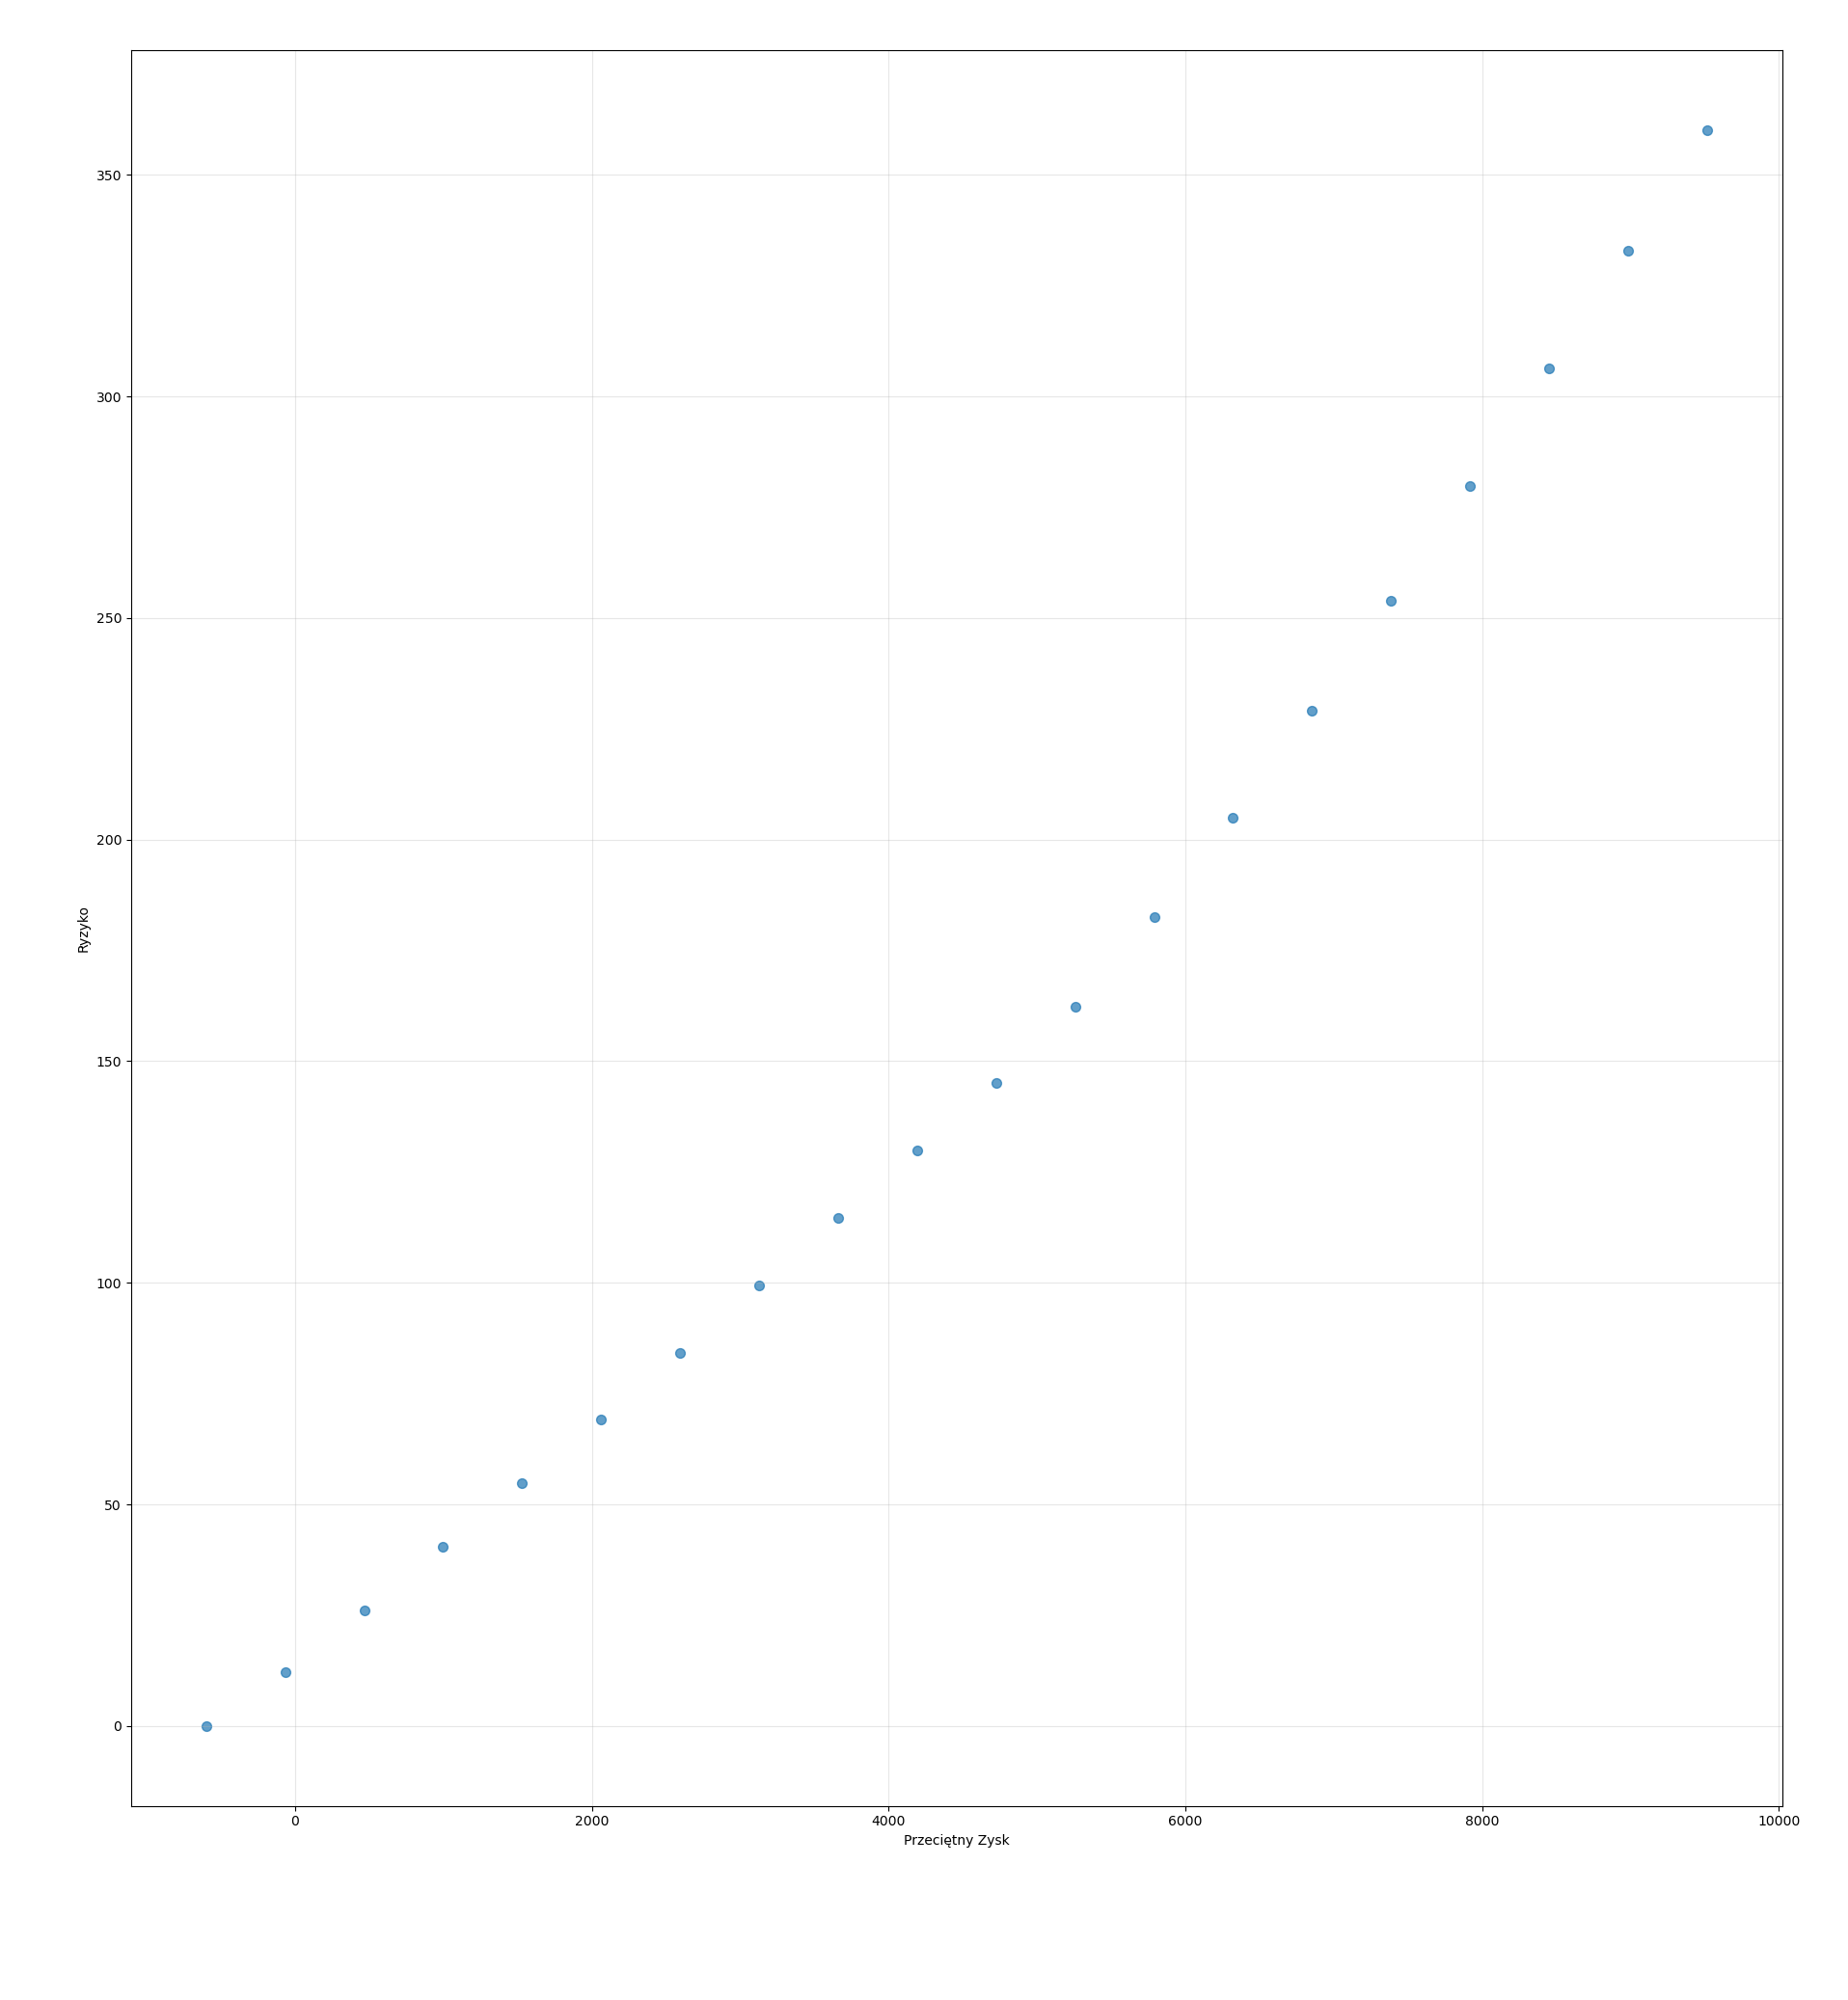
\includegraphics[width=0.8\textwidth]{graphics/ryzyko_zysk_wykres.png}
\caption{Obraz zbioru rozwiązań efektywnych w przestrzeni ryzyko-zysk}
\label{fig:profit-risk}
\end{figure}

\subsection{Rozwiązania efektywne minimalnego ryzyka i maksymalnego zysku}
\addcontentsline{toc}{subsection}{Rozwiązania efektywne minimalnego ryzyka i maksymalnego zysku}

\begin{table}[H]
\label{tab:min-max}
  \caption{Rozwiązania maksymalnego zysku i minimalnego ryzyka}
  \centering
  \begin{tabular}{l*{4}{c}}
  
  	\hline
              			& Miara zysku & Miara ryzyka \\
	\hline
	Maksymalizacja zysku	& 9515.80 zł & 360.18 zł \\
	Minimalizacja ryzyka   	& -600.00 zł & 0.0 zł \\ 
	\hline
	
	\end{tabular}
	\end{table}
	
Rozwiązanie zadania jednokryterialnego maksymalizacji zysku charakteryzuje się również maksymalizacją poziomu ryzyka, podczas gdy zadanie 
minimalizacji ryzyka bez nałożenia ograniczeń na poziom zysku prowadzi do ujemnego wyniku finansowego (straty) wynikającego z rezygnacji ze 
sprzedaży oraz ponoszenia kosztów utrzymania obligatoryjnych zapasów magazynowych.

\subsection{Dominacja stochastyczna wybranych rozwiązań efektywnych}
\addcontentsline{toc}{subsection}{Dominacja stochastyczna wybranych rozwiązań efektywnych}
Do weryfikacji relacji dominacji stochastycznej pierwszego rzędu (FSD) zostały wybrane 3 rozwiązania efektywne modelu: Scenariusze 1, 2 i 3,
Parametry charakteryzujące średni zysk i miarę ryzyka dla analizowanych rozwiązań przedstawiono w tabeli \ref{tab:abc}. 
Implementacja parametrów oraz modelu została zawarta w plikach wdwr25406-4.dat i wdwr25406-4.mod - skrypty przeznaczone dla solvera CPLEX 
służące do generowania informacji o zysku i ryzyku w ramach poszczególnych scenariuszy.

\begin{table}[H]
  \label{tab:abc}
  \caption{Scenariusze wybrane do analizy dominacji FSD}
  \centering
  \begin{tabular}{lccc}
  	\hline
              			& 1 & 2 & 3 \\
	\hline
	Ograniczenie minimalnego zysku	& 8450.97 zł & 8983.38 zł & 9515.79 zł\\
	Średni zysk   	& 8451.02 zł & 8983.40 zł & 9515.80 zł\\
	Miara ryzyka   	& 306.38 zł & 332.93 zł & 360.18 zł\\ 
	\hline
	\end{tabular}
\end{table}

Aby określić relacje dominacji między wybranymi rozwiązaniami w kontekście FSD, zbudowano odwrotne dystrybuanty 
dla obydwu analizowanych kryteriów. Rysunek \ref{fig:FSD-profit} prezentuje odwrotną dystrybuantę rozkładu średniego 
zysku w poszczególnych scenariuszach dla trzech wybranych rozwiązań efektywnych. Z analizy wykresu wynika, 
że rozwiązanie dla scenariusza 3 przewyższa rozwiązania scenariusza 1 i 2 w kontekście dominacji stochastycznej pierwszego rzędu, 
oznaczając, że dla każdego scenariusza wartość zysku osiągana przez decyzję 3 jest wyższa niż 
odpowiadające jej wartości dla decyzji 1 i 2. Jednocześnie rozwiązanie 2 dominuje nad rozwiązaniem 1
w sensie dominacji stochastycznej pierwszego rzędu.

\begin{figure}[H]
\centering
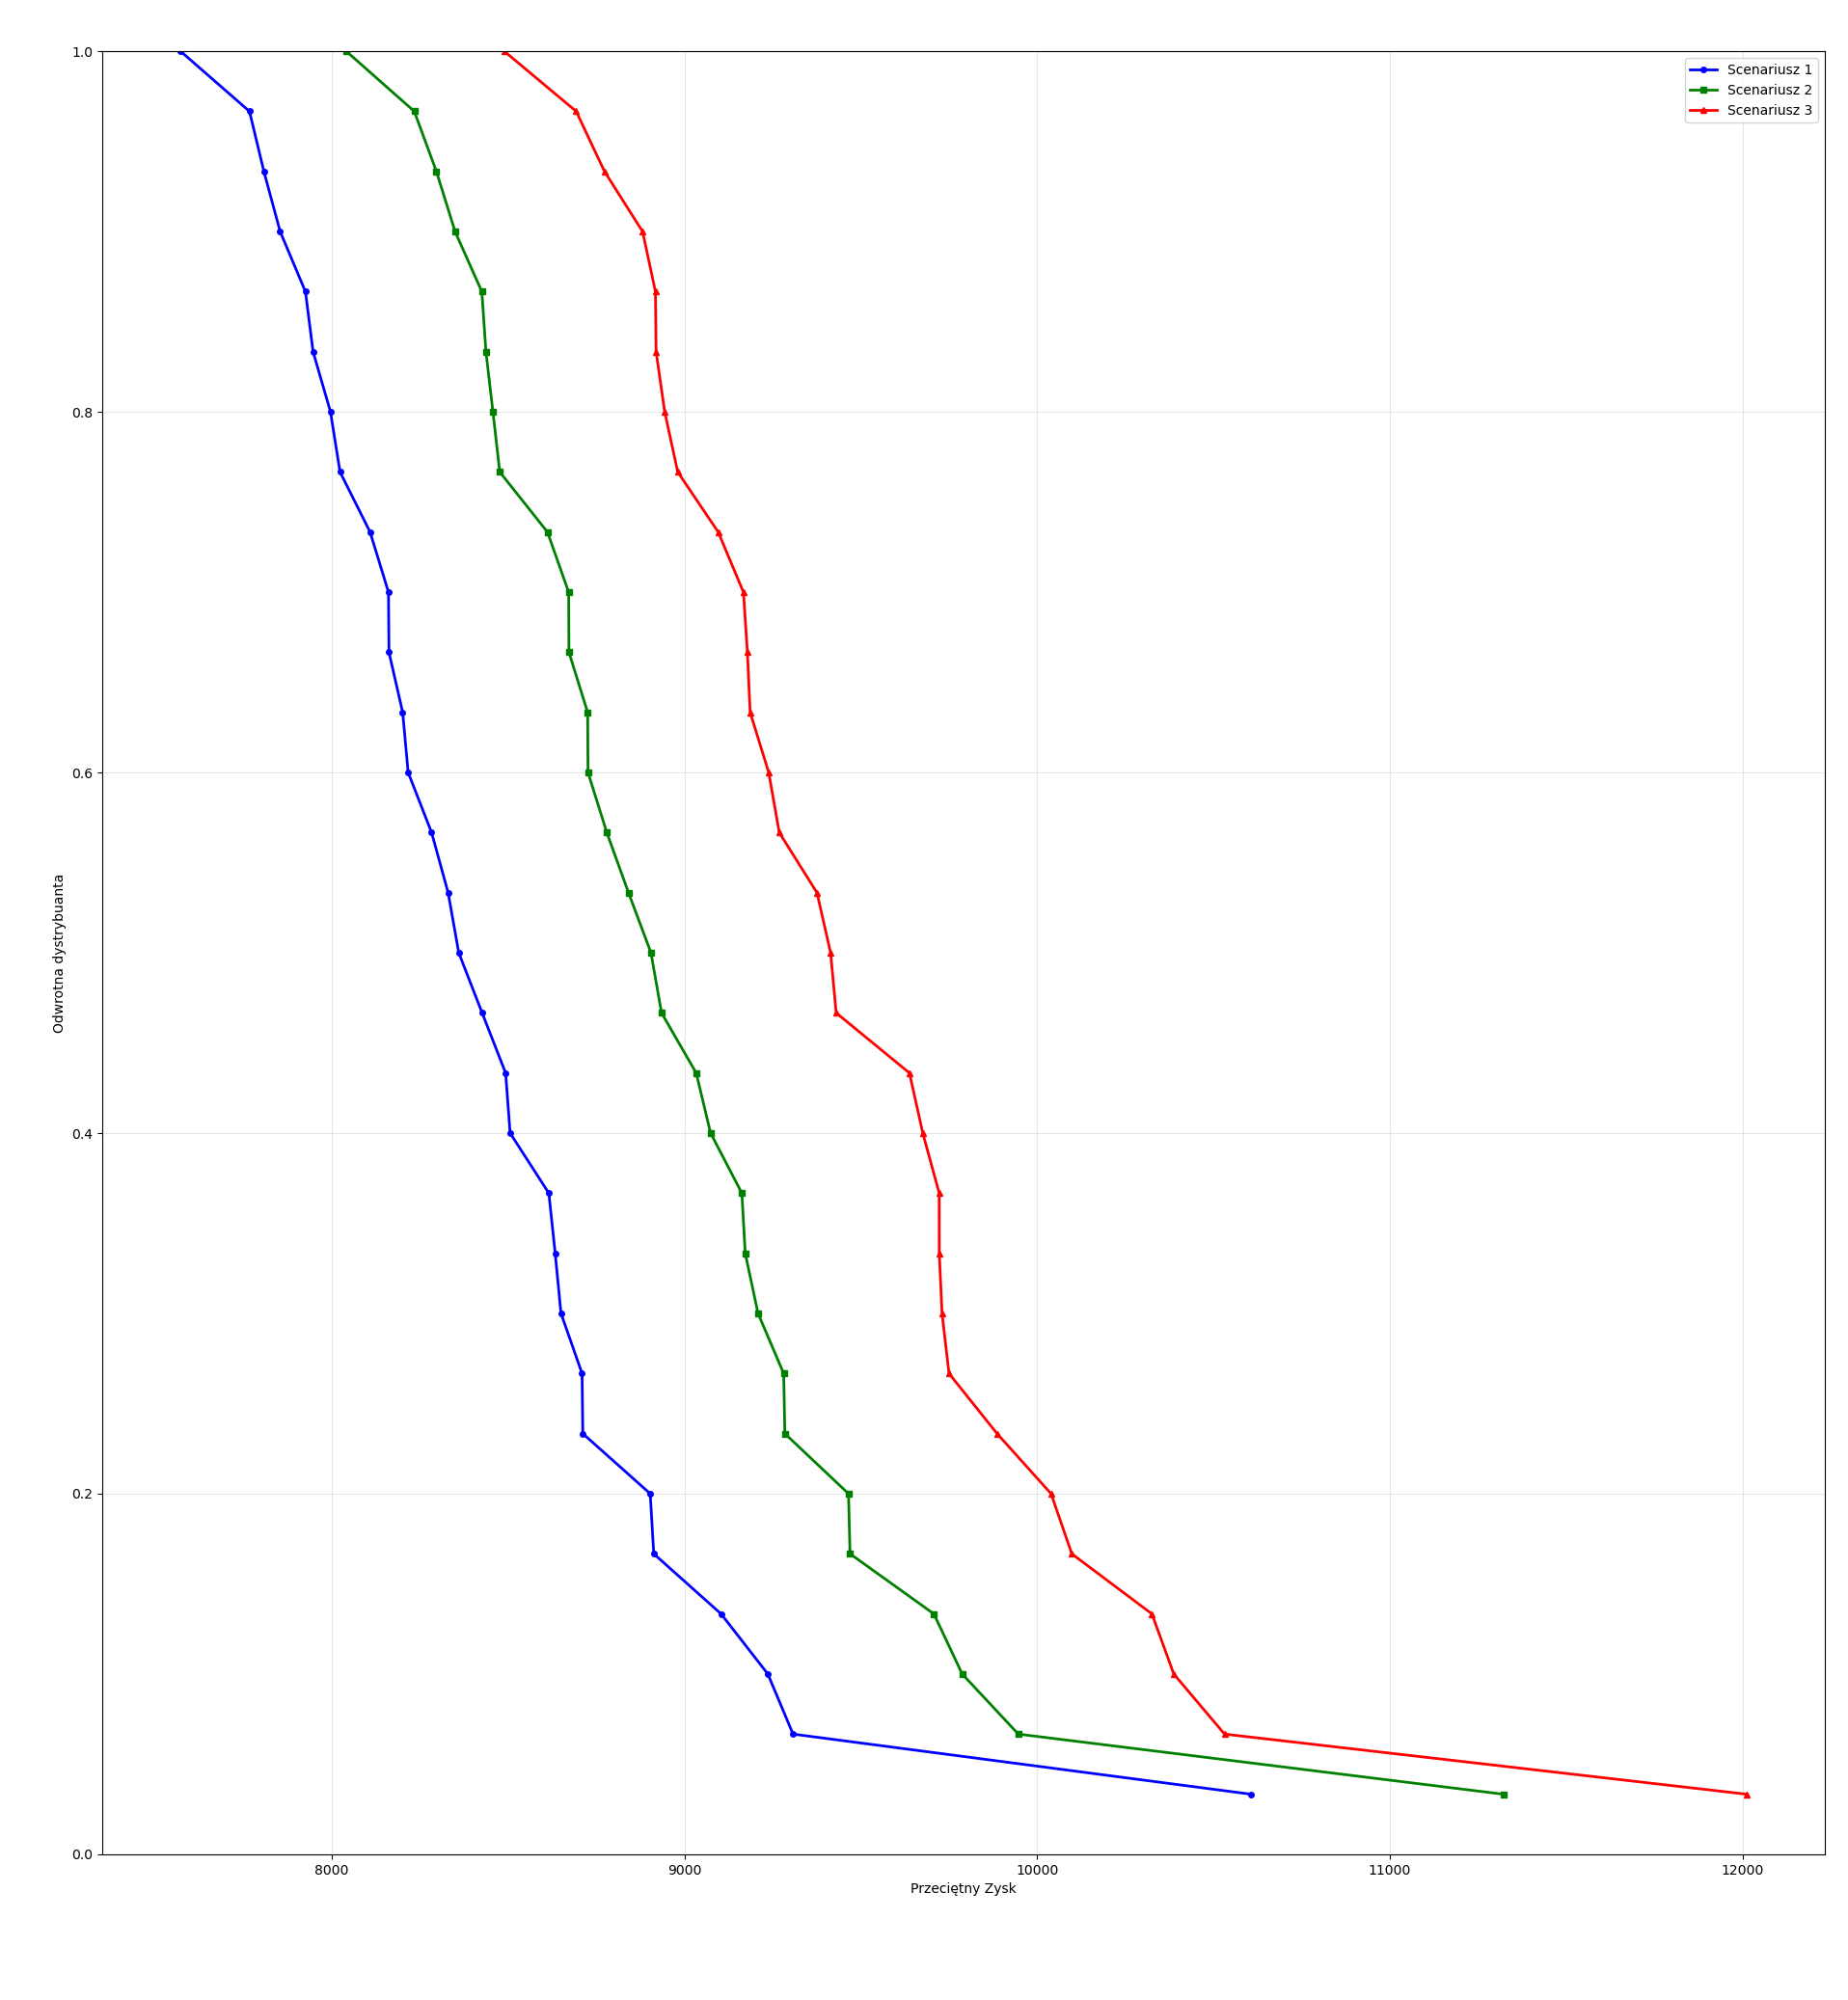
\includegraphics[width=\textwidth]{graphics/zysk_dystrybuanta.png}
\caption{Odwrotna dystrybuanta rozkładu średniego zysku między scenariuszami}
\label{fig:FSD-profit}
\end{figure}
Rysunek \ref{fig:FSD-risk} prezentuje odwrotną dystrybuantę rozkładu średniej różnicy Giniego jako miary ryzyka dla 
tych samych trzech rozwiązań efektywnych. W zakresie miary ryzyka rozwiązanie 1 charakteryzuje się dominacją 
nad rozwiązaniami 2 i 3, rozwiązanie 2 wykazuje również jednoznaczną dominację względem rozwiązania 3. 

\begin{figure}[H]
\centering
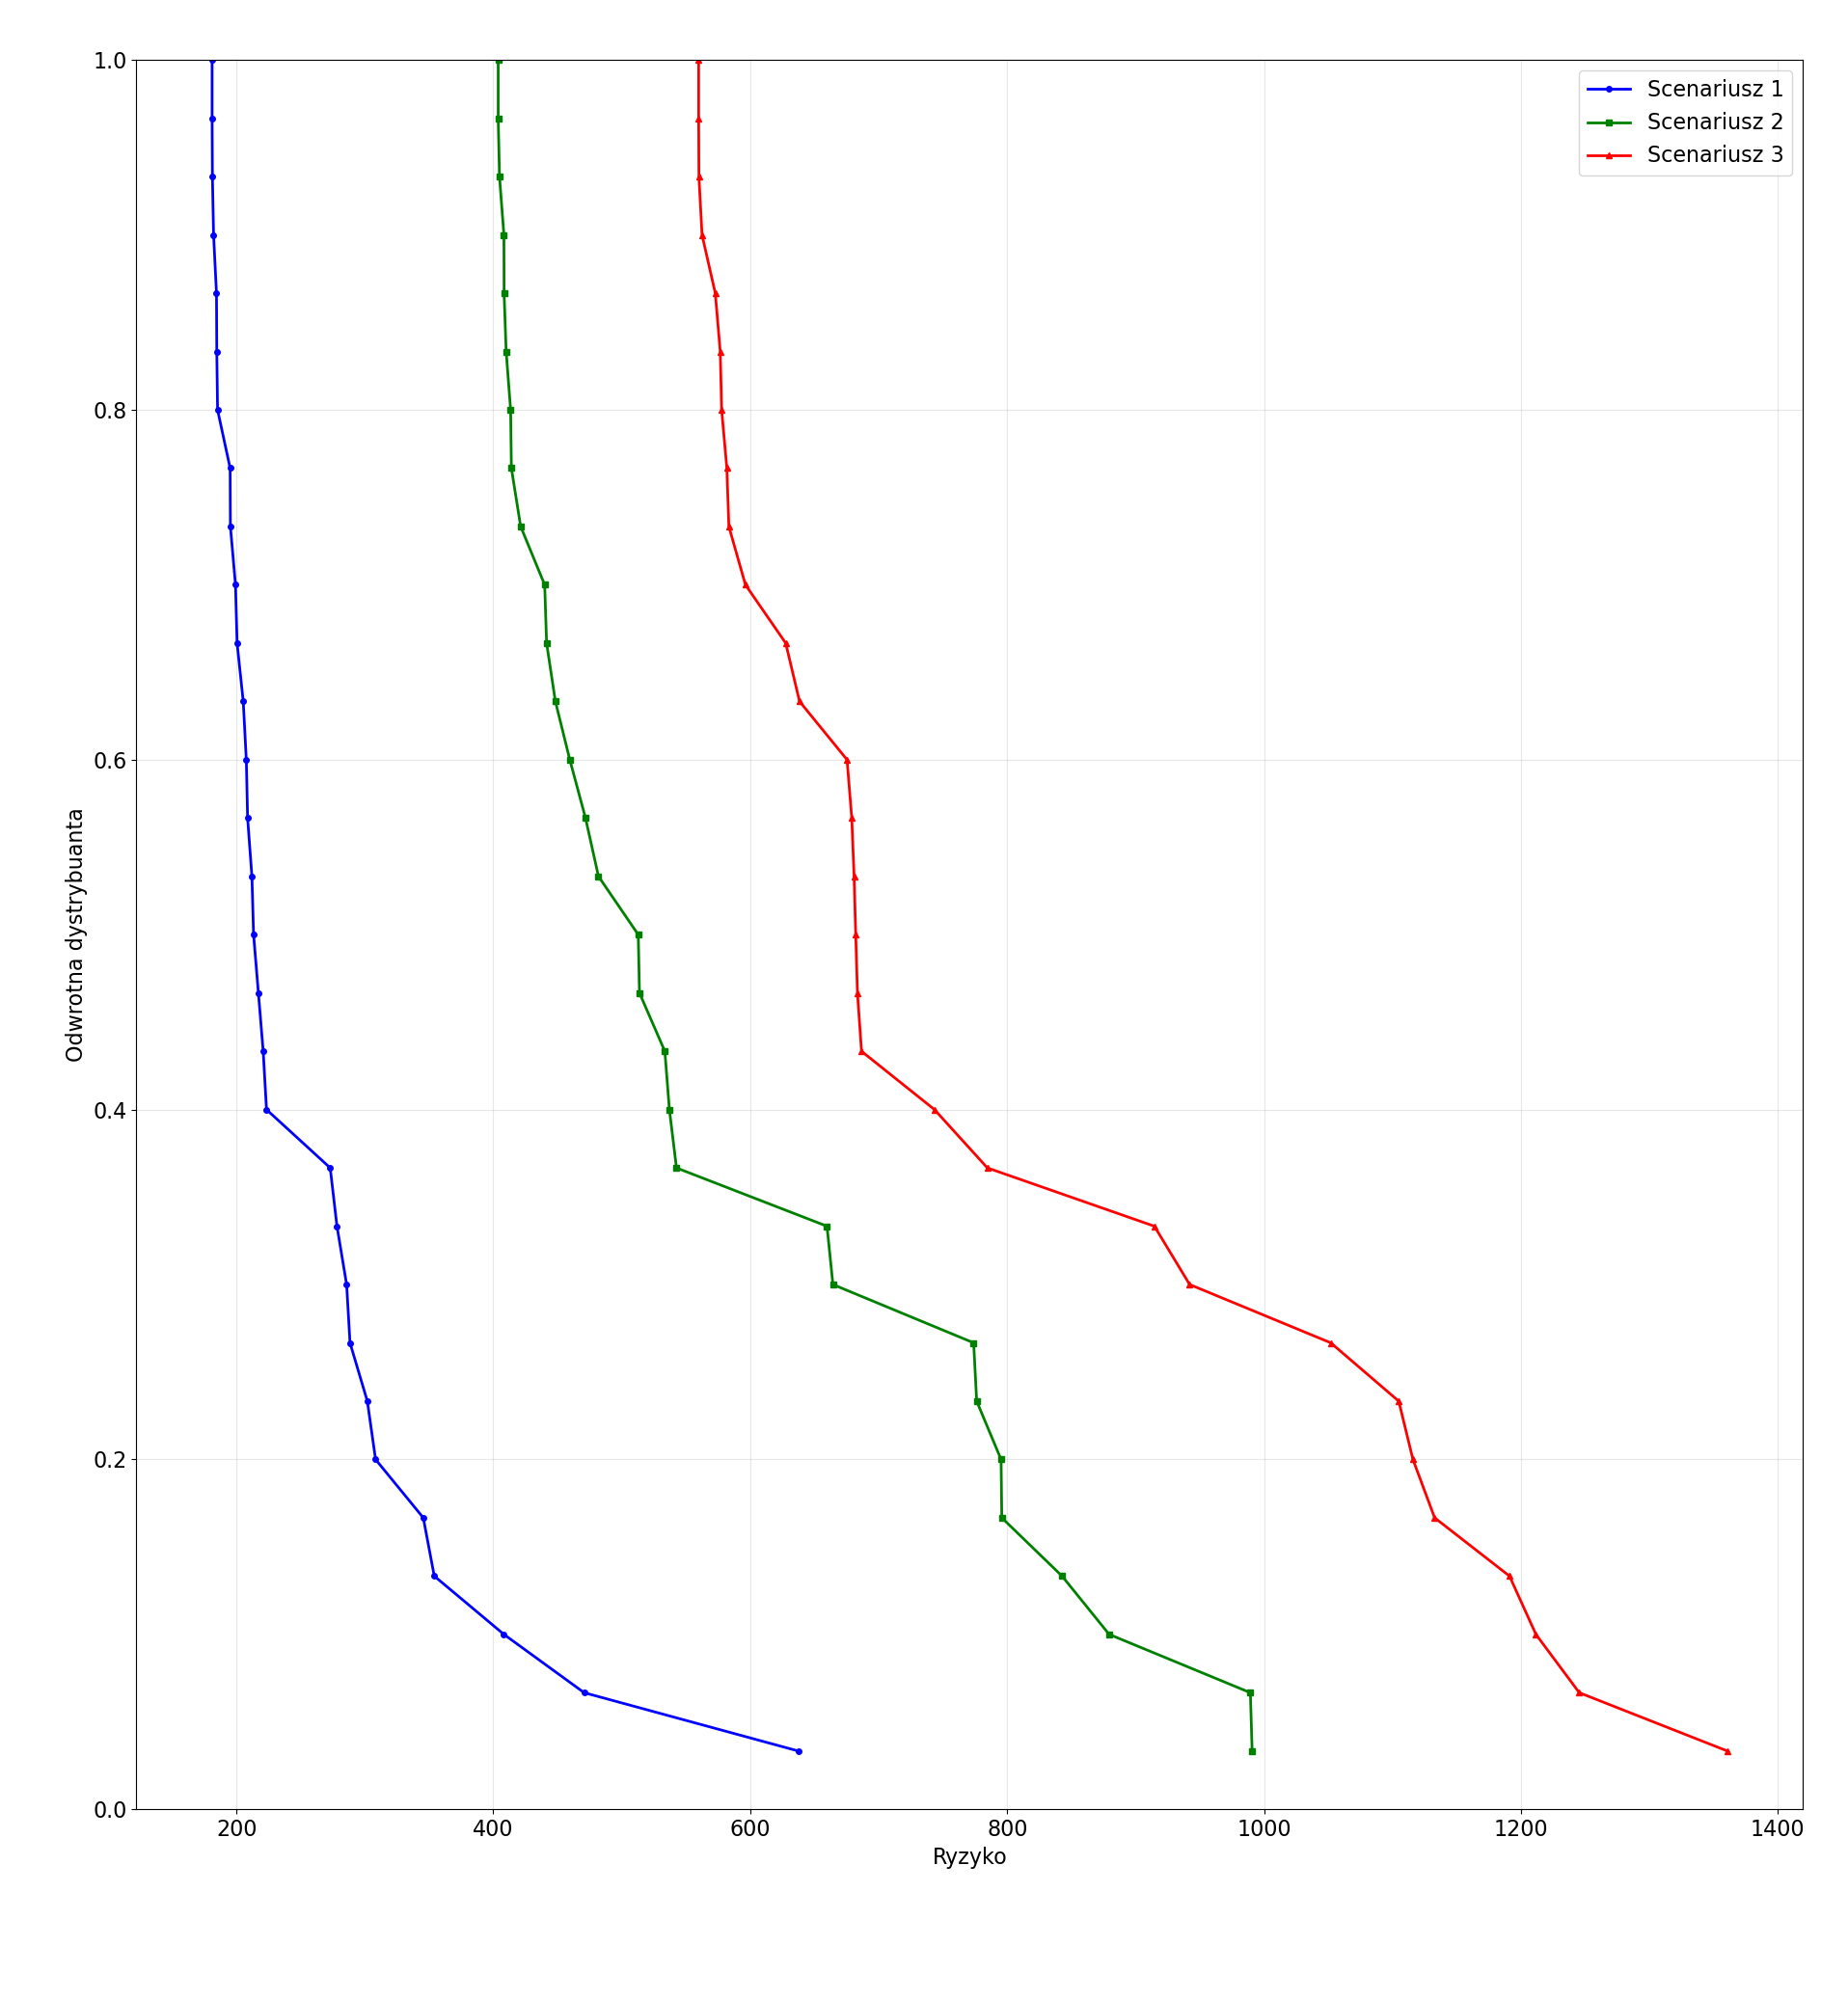
\includegraphics[width=\textwidth]{graphics/ryzyko_dystrybuanta.png}
\caption{Odwrotna dystrybuanta rozkładu średniej różnicy Giniego między scenariuszami}
\label{fig:FSD-risk}
\end{figure}


\end{document}